
\documentclass[14pt]{memoir}


% Lorem Ipsum Text
\usepackage{lipsum}

% Section and Figure Numbering
\renewcommand\thesection{\arabic{section}}
\usepackage{chngcntr}
\counterwithout{figure}{chapter}
\counterwithout{table}{chapter}

% Referencing Commands
\newcommand{\refsec}[1]{\hyperref[sec:#1]{Section~\ref{sec:#1}}}
\newcommand{\reffig}[1]{\hyperref[fig:#1]{Figure~\ref{fig:#1}}}
\newcommand{\reftab}[1]{\hyperref[tab:#1]{Table~\ref{tab:#1}}}

%TiKz
\usepackage{tikz}
\usetikzlibrary{arrows}
\usetikzlibrary{shapes}

%SidewaysFigure
\usepackage{rotating}

% CMU sans serif font.
\usepackage[T1]{fontenc}
\renewcommand*\familydefault{\sfdefault}

% Hyperlinks
\usepackage{hyperref}
\hypersetup{
    colorlinks=true,       % false: boxed links; true: colored links
    linkcolor=black,          % color of internal links (change box color with linkbordercolor)
    citecolor=black,        % color of links to bibliography
    filecolor=blue,      % color of file links
    urlcolor=blue           % color of external links
}

% APA 6 citation and bibliography style % Note: Must be loaded after hyperref
\usepackage{apacite} 

% Abbreviations
\usepackage{glossaries}
\makeglossaries

\newacronym{pisa}{PISA}{Programme for International Student Assessment}
\newacronym{oecd}{OECD}{Organisation for Economic Co-operation and Development}
\newacronym{stem}{STEM}{Science, Technology, Engineering and Mathematics}
\newacronym{fmri}{fMRI}{functional magnetic resonance imaging}
\newacronym{naplan}{NAPLAN}{National Assessment Program --- Literacy and Numeracy}
\newacronym{mars}{MARS}{Maths Anxiety Rating Scale}
\newacronym{mas-r}{MAS-R}{Maths Anxiety Scale --- Revised}
\newacronym{ptsd}{PTSD}{Post-Traumatic Stress Disorder}



\title{A Longitudinal Study of a Multifaceted Intervention for Maths Anxiety}
\author{Lyron Winderbaum}



\begin{document}



\maketitle



\begin{abstract}

The longterm effectiveness of maths anxiety interventions is in some question, and this is a recognised need for research in this area \cite{Pellicioni2016,Chang2016}. Several critical links between maths anxiety and performance have been identified, but \citeA{Ramirez2018} propose a convincing model that fits these links together into a cycle. The model of \citeA{Ramirez2018} imples that interventions targeting only a single link may be ineffective in the longterm, as even if the targetted link is disrupted, the others will restablish the cycle. I propose a longitudinal study of an intervention targetting multiple links simultaneously. This multifaceted approach has not been trialled to my knowledge, and if it successfully disrupts the cycle it has the potential to yield improved longterm outcomes.

\end{abstract}
% 100-150 words


\pagebreak
\glsresetall
\section{Literature Review}


\subsection*{Why is Maths Anxiety Important?}

Maths anxiety is hugely prevalent, the 2012 \gls{pisa} report states that across \gls{oecd} countries, over 30\% of 15 year old students ``get very nervous doing mathematics problems'', and over 60\% of students ``worry about getting poor grades in mathematics''  \cite{PISA2013}. As teachers our foremost concern should be for the wellbeing of our students. It has been shown that students with a high level of maths anxiety often literally experience the anticipation of a maths task as visceral pain \cite{Lyons2012pain}. There is a clear and overwhelming moral imperative (and ethical duty of care) on us to do everything in our power to protect students in our care from maths anxiety.

Even if the wellbeing issue was not enough, there is also a clear maths anxiety-performance connection, and all the stakeholders in a students academic success in maths. One example of this is highlighted by \citeA{Foley2017} who juxtaposes the internationally rising demand for \gls{stem} professionals with the negative correlation between maths anxiety and performance shown in the 2012 \gls{pisa} report \cite{PISA2013} to highlight the relevance of addressing maths anxiety in filling this demand. The relationship between maths anxiety and maths-qualified professionals in the workforce is supported throughout the literature: when a student has low self-concept (correlated with high maths anxiety), they will tend not to enroll in maths beyond the minimum requirements for graduation \cite{Ashcraft2007book}, and students affect towards maths can predict their university major \cite{LeFevre1992}. Beyond this example, the list of stakeholders in a students academic success in maths goes on and on: parents; the student's themselves; schools (which are often funded based on the results of standardised testing such as \gls{naplan}), and teachers amongst them. 



\subsection*{Frameworks for Understanding Maths Anxiety}.

Only a few studies focus on maths anxiety itself (primarily \gls{fmri} studies such as those of  \citeA{Young2012} or \citeA{Lyons2012pain}). Instead the bulk of the literature is focused on the maths anxiety-performance link.  Specifically, there seem to be two distinct theories being pursued and I will adopt the terminology of \citeA{Ramirez2018} to describe them: the ``Disruption Account'' and the ``Reduced Competency Account''. \citeA{Ramirez2018} go on to make a convincing argument that although these two theories might seem to compete, they are not actually mutually exclusive and instead quite compatible with each other. \citeA{Ramirez2018} suggests a third ``Interpretation Account'' which encapsulates observations made by both lines of research, see \reffig{ramirez}.

\begin{figure}[b]
\begin{center}
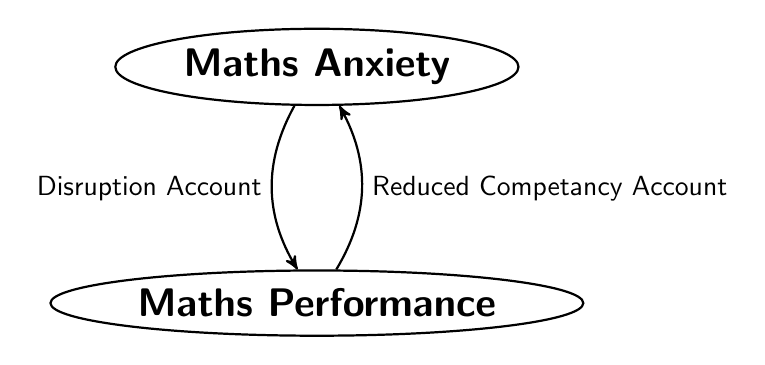
\begin{tikzpicture}[->,>=stealth',auto,node distance=3cm,thick,main node/.style={ellipse,draw,font=\sffamily\Large\bfseries}]
  	\node[main node] (a) {Maths Anxiety};
 	\node[main node] (b) [below of=a] {Maths Performance};

	\path	(a) edge[bend right] node [left] {Disruption Account} (b)
		(b) edge[bend right] node [right] {Reduced Competancy Account} (a);
\end{tikzpicture}
\end{center}
\caption{The Interpretation Account of Ramirez et al. (2018) for the maths anxiety-performance link showing how the Disruption Account and the Reduced Competency Account can be compatible.
\label{fig:ramirez}}
\end{figure}

First, a little more detail on the existing theories. The ``Disruption Account'', spearheaded by the work of Ashcraft et al., is centered around the concept of working memory \cite{Ashcraft2001, Ashcraft2007}. Specifically that anxiety about maths takes up students working memory, which prevents them from using that working memory to complete maths tasks and thereby impacts their performance. The ``Reduced Competency Account'' on the other hand proposes the opposite causality: that lower ability in maths leads to negative experiences associated to maths, which in turn cause maths anxiety to develop. There is also a significant body of work to support this hypothesis, including the milestone meta-analysis of \citeA{Hembree1990} and the longitudinal study of \citeA{Ma2004} which found that although past maths anxiety was correlated with future maths performance it was a small effect, while past maths performance had a strong effect on future maths anxiety.



\subsection*{Complexities in Finding Effective Interventions}

These theoretical views are of course broad oversimplifications of what is an incredibly complex and interconnected topic. They also imply very different approaches for intervention. The ``Reduced Competency Account'' would imply interventions to boost maths performance and hence allow students to experience success in math should also help to reduce maths anxiety. The results of  \citeA{Supekar2015} seem to support this hypothesis as when students are given an intensive 8-week tutoring program to boost their maths skills, this is associated to a reduction in maths anxiety. The earlier work by \citeA{Faust1996} further supports this by demonstrating an anxiety-complexity effect in which low and high maths anxiety groups performed similarly on low complexity problems, but in high complexity problems the high anxiety groups performance was impacted. On the other hand, \citeA{Jansen2013} showed that it is not neccessarily that simple, by showing that when students experience more success they attempt more problems and perform better. However their improved performance is almost completely predicted by the number of problems they attempted, not their experience of success, and their level of maths anxiety was not affected in a significant way which raises a lot of interesting but unanswered questions about this approach. 
	
On the other side of attempted interventions are those in line with the ``Disruption Account'', in which the maths anxiety itself is addressed in the hopes that will free up extra working memory and hence boost students performance.  \citeA{Park2014} demonstrate a direct and successful attempt at this in which they used expressive writing exercises to help guide students self-perceived narratives about their maths experiences and thereby reduce their maths anxiety. Notably the approach of \citeA{Park2014} is in line with successful treatments for clinical anxiety disorders (see \citeA{McNally2007, Becker2007,Foa2005}). Another approach that has shown success in this vein does not attempt to directly reduce the anxiety experienced, but rather reappraise it's symptoms \cite{Jamieson2016}. This is another technique from clinical psychology in which stress is reconceptualised as a coping tool, an evolutionary method for heightening performance in response to a challenge to be overcome, instead of a symptom of exposure to something to be feared and avoided. This change in the perspective of stress is also very much in line with the ``Interpretation Account'' of \citeA{Ramirez2018}.

The work of \citeA{Wang2015} showed the role that intrinsic motivation has mediating the relationship between maths anxiety and performance, and suggested the importance of a mindset centred on viewing the process of learning maths as one of ``productive struggle''. This reconceptualisation to a `productive struggle' model is supported by other literature as well, \citeA{Lin-Siegler2016} exposes students in a classroom to struggles experienced by famous scientists in order to help normalise the concept of productive struggle, and \citeA{Hiebert2007} discuss the importance of this same concept in a maths context.

One of the implications of the ``Interpretation Account'' is that if an intervention targets only one of these two possible links in the cycle (see \reffig{ramirez}), the cycle may re-establish itself after the intervention is over and negate any potential longterm effects. However there is only a very limited amount of research out there on such longterm effects, and several authors have discussed the need for further research into this \cite{Pellicioni2016,Chang2016}. My hypothesis is that a multi-faceted approach targetting both directions simultaneously could disrupt the cycle shown in \reffig{ramirez} and result in significant longterm effects.



\section{Research Proposal}

I propose a multifaceted intervention in which multiple links in the cycle (see \reffig{ramirez}) are attacked simultaneously to disrupt the maths anxiety-performance link. I hypothesise that this approach will result in a more longlived effect on both students wellbeing (anxiety mediated by self-concept) and maths performance. The four facets of the proposed intervention are:
\begin{itemize}
	\item An intensive tutoring program to boost students math abilities, similar to the approach of \citeA{Supekar2015}.
	\item Coaching around reappraisal of physiological signs of stress (increased heart rate, sweaty palms, etc.) similar to the approach of \citeA{Jamieson2016}.
	\item Guided expressive writing, similar to the approach of \citeA{Park2014}.
	\item Coaching perception of learning maths towards a viewpoint including ``productive struggle'' \cite{Hiebert2007}.
\end{itemize}

The intensive tutoring program will be delivered by separate tutors, but the other interventions will be delivered by the classes regular teachers. Hence, a critical component to this design will be a professional development course running ``Teacher Coaching Sessions'' throughout the study, in which the classroom teachers will be explained the principles of the interventions, and more importantly will be able to ask questions in an ongoing manner throughout the study to continue to modify and improve their pedagogy.

\subsection*{Instruments for Measuring Maths Anxiety}

In order to track the effectiveness of these interventions, we will be collating assessment results as a measure of performance, but will also want to measure maths anxiety and maths affect/ self-concept. Significant work has been done over the years to develop psychometrics to measure maths anxiety, almost exclusively consisting of self-reporting surveys (with the exception of some more modern \gls{fmri} work, such as that of \citeA{Lyons2012}). We will use a recently developed scale: the \gls{mas-r} of \citeA{Bai2009}, which has been shown to be remarkably self consistent by incorporating both positive and negative affect items \cite{Bai2011}. It is short, easy to implement, and cheap in comparison to \gls{fmri} methods. In order to measure maths self-concept, \citeA{Jansen2013} modified the Perceived Competence Scale for Children of \citeA{Harter1982} to measure ``Math Competance''. The methodological process imployed by \citeA{Jansen2013} was quite rigorous and so we will use their instrument, or a minor modification thereof (we will do it in English), to measure maths self-concept.



\subsection*{Timeline}

Each intervention will be introduced sequentially, with at least a 3-week gap between them. This will allow for a multivariate time-varying autoregressive model to seperate individual effects should there be any. 

 \begin{sidewaysfigure}
 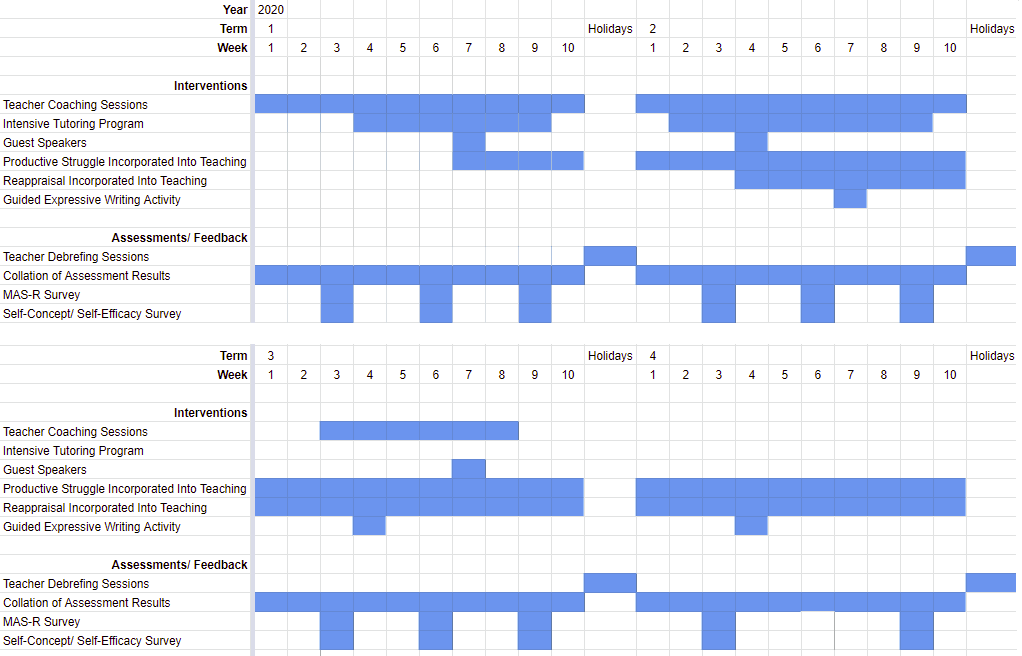
\includegraphics[scale=0.7]{Gantt_Chart.PNG}
\caption{Gantt Chart \label{fig:gantt}}
\end{sidewaysfigure}

\begin{table}[p]
\begin{center}
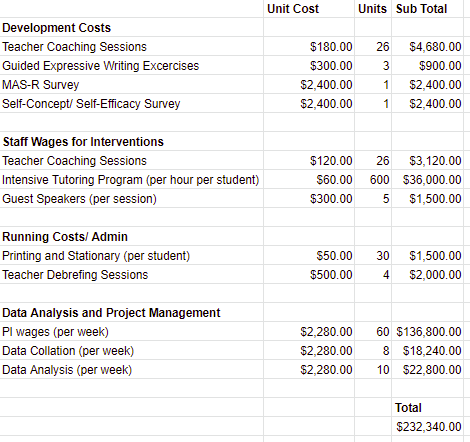
\includegraphics[scale=1.2]{Budget.PNG}
\end{center}
\caption{Budget \label{tab:budget}}
\end{table}

The proposed timeline for 2020 is shown in \reffig{gantt} in which the bulk of the study will be conducted. The key points can be split into two conceptual levels. The first conceptual level is the timeframe for the interventions:
\begin{itemize}
	\item 2019: Assessment instruments and instruction programs will be developed and fine-tuned.
	\item 2020 Term 1 Week 1: Teacher coaching sessions begin and continue until the end of Term 2.
	\item Term 1 Week 4: Intensive tutoring program begins and continues until Term 3, 6 weeks worth in Term 1, 8 in Term 2, and 6 in Term 3.
	\item Term 1 Week 7: Guest Speaker on productive struggle, and teachers start implmenting productive struggle program which will continue for the the remainder of the year. 
	\item Term 2 Week 4: Guest speaker will return, refresh productive struggle talk and give reappraisal talk. Teachers will begin reappraisal program which will continue for the remainder of the year.
	\item Term 2 Week 7: Expressive writing excercises once per term for the remainder of the year.
	\item Term 3 Week 7: Guest Speakers return to reinforce productive struggle and reappraisal concepts.
	\item 2021: Students will return to ordinary classes.
\end{itemize}

The second conceptual level is the streams of ongoing primary data collection throughout:
\begin{itemize}
 	\item  During school holidays there will be teacher debrefiing sessions in which the teachers will be asked to provide feedback on their perspectives on the effects of the interventions.
 	\item Academic results of students will be collated for an entire three year 2019-2021 period.
 	\item Students will complete self-surveys on both maths anxiety, and maths self-concept the year prior, during, and the year after the interventions. These will occur before and after the introduction of each facet of the intervention, allowing for multivariate interaction effects to be modelled.
 	\item The expressive writing tasks will yield written work from each student describing their narative view of their journey learning maths, which can also be used to assess their self-concept/ efficacy in a deeper way.
\end{itemize}

This ongoing data will be fed back into the teacher coaching sessions to further improve practice, and this will be modelled during the data analysis stage with an autoregressive model to represent the time-dependancies in the data collection.

\subsection*{Budget}

This research is predicated on collaborating with a school and the maths faculty therein, and the leadership team at the school being on board. The budget proposed above (see \reftab{budget}) presupposes $30$ student participants either in one class or split accross two classes, $1-2$ teacher participants, and for the entire study to be performed over the three year period 2019-2021. Should additional funding be made available, it would be possible to extend the study to include a larger sample of students and teachers, and to continue monitoring the students into 2022-2023, which would offer very valuble additional data on the longer term effects of the interventions.

\section{Ethics Issues}

\begin{itemize}
	\item Teacher and student participants, parents, and school leadership will be given full experimental details prior to commencement. 
	\item All published results will be fully anonymised.
	\item Students and parents will have the option to opt-out at any time. Any student that wishes to be withdrawn will be moved to a class not participating in the study. Withdrawn data will be ommitted from all analyses, the only remaining trace a note of the total number of students that were withdrawn.
	\item Teachers will have complete autonomy running their classes, and will have the right to stop the study at any time should they beleive it to be causing any harm (emotional, or academic) to the students.
	\item All content addressing anxiety and other sensitive topics will include appropriate trigger warnings. Furthermore a school councillor and a ``cooling off space'' will be available at all times should a student find themselves in distress.
\end{itemize}


\section{Executive Summary}

I propose a longitudinal study of a multifaceted intervention to address maths anxiety and disrupt the maths anxiety-performance link that will have long lasting positive impacts on students mathematical self-concept as well as their performance. This proof of principle study will not only contribute to the broader maths anxiety field by providing much needed longitudinal data, but also offers to provide evidence of a broader unifying theory of the maths anxiety-performance link, i.e. the ``Interpretation Account'' of \citeA{Ramirez2018} by showing that a combined multi-target intervention can produce tangible longterm effects that single-target interventions may not be capable of doing. Furthermore, this study will demonstrate how the use of high-dimensional multivariate time-varying autoregressive models can be used to provide meaningful insights into interaction effects between multiple factors impacting on students in a complex and constantly changing enviornment. 





%\subsection*{Maths Anxiety as Distinct from General Anxiety}
%
%The existence of maths anxiety as ``emotional disturbances in the presence of mathematics'' has been noted as early as the 1950's, \citeA{Dreger1957} even postulated that what he tentatively designated ``Number Anxiety'' and later became to be known as Maths Anxiety could be a distinct syndrome from general anxiety. Later the landmark meta-study of \citeA{Hembree1990} supported this hypothesis, showing a correlation of only $0.38$ between maths anxiety and general anxiety. In more recent times, this hypothesis has also been confirmed by \citeA{Young2012} using \gls{fmri} to show that the brain activity in a person experiencing maths anxiety is measurably distinct from that in a person suffering general anxiety. These later studies, as well as the the work of \citeA{Kazelskis2000} and more, have also delineated maths anxiety from test anxiety, and these different anxieties exisitng as meaningfully distinct constructs is now quite well accepted. For more on the history of maths anxiety, \citeA{Pellicioni2016} offers a more detailed review.



\printglossaries

\glsresetall
\bibliographystyle{apacite}
\bibliography{citations} 

\end{document}


